\documentclass[aspectratio=169]{beamer}
\usetheme[]{msubeamer}
\usepackage[T1]{fontenc}
\usepackage[backend=bibtex,sorting=none]{biblatex}
\addbibresource{mybeamer.bib} 
\usepackage{multirow}
\usepackage[ruled,linesnumbered]{algorithm2e}
\usepackage{algorithmic}
\usepackage{subfigure}
\usepackage{float}
\usepackage{epstopdf}
%\setbeamerfont{footnote}{size=\small}
\begin{document}
	
%%%%%%%%%%%%%%%%%%%%%%%%%%%%%%%%%%%%%%%%%%%%%%%%%%%%%%%%%
\xdefinecolor{dred}{rgb}{0.6, 0.0, 0.0}
\setbeamercolor{math text}{fg=dred}
%%%%%%%%%%%%%%%%%%%%%%%%%%%%%%%%%%%%%%%%%%%%%%%%%%%%%%%%%

\title[Adam-CBO]{A consensus-based global optimization method with adaptive momentum estimation}
\maketitleframe
\begin{frame}
\frametitle{Machine learning tasks}

Highly nonconvex unconstrained optimization problem
\begin{align*}
x^* = \arg\min_{x\in \mathbb{R}^d} f(x)
\end{align*}
with the loss function
\begin{equation*}
f(x) = \frac{1}{n}\sum_{i=1}^n f_i(x) = \frac{1}{n}\sum_{i=1}^n\|\mathcal{N}_x(\hat{x})-\hat{y}\|
\end{equation*}
\begin{itemize}
	\item[] $x$ is the parameter vector
	\item[] $\mathcal{N}_x$ represents a neural network representation
	\item[] $(\hat{x}_i,\hat{y}_i)_{i=1}^n$ is a set of labeled data
	\item[] $\|\cdot\|$ is the $L^2$ distance
	\item[] \textcolor{red}{$d\gg 1$}
\end{itemize}

\end{frame}

\begin{frame}<beamer>
\frametitle{\textbf{Outline}}
\tableofcontents[]
\end{frame}

\section{Optimization methods: Zero-order or first-order?}

\begin{frame}
\frametitle{First-order methods}

\begin{itemize}
	\item gradient descent method
	\begin{equation*}
	x^{t+1} = x^t - \alpha \nabla f(x^t)
	\end{equation*}	
	with $\alpha$ being the learning rate
	\item stochastic gradient descent (SGD) method
	\begin{equation*}
		x^{t+1} = x^t - \alpha \nabla f_i(x^t)
	\end{equation*}	
	\item SGD method with momentum term \footfullcite{Qian1999Jan}
	\begin{align*}
		&x^{t+1} = x^t - m^t\\
		&m^t = -\gamma m^{t-1} + \alpha \nabla f_i(x^t)
	\end{align*}
\end{itemize}

\end{frame}

\begin{frame}
\frametitle{Cont'd}

\begin{itemize}
	\item Adaptive momentum method (Adam) \footfullcite{kingma2014adam} 
	\begin{align*}
	&x^{t+1} = x^t - \gamma \frac{\hat{m}^t}{\sqrt{\hat{v}^t}+\epsilon}\\
	&m^t = \beta_1 m^{t-1} + (1-\beta_1) \nabla f(x^t), \quad \hat{m}_t = \frac{m_t}{1-\beta_1^t}\\
	&v^t = \beta_2 v^{t-1} + (1-\beta_2) \nabla^2 f(x^t), \quad \hat{v}_t = \frac{v_t}{1-\beta_1^t}
	\end{align*}
	where $0<\beta_1,\beta_2<1$
\end{itemize}
\end{frame}

\begin{frame}
\frametitle{First-order methods}

\begin{itemize}
	\item mostly have problems with loss functions containing large noise or non-differentiable units
	\item gradient tends to explode or vanish as the neural network gets deeper\footfullcite{hanin2018neural}
	\item are easily influenced by the loss landscape\footfullcite{liu2020bad}
\end{itemize}

\end{frame}

\begin{frame}
	\frametitle{Zero-order methods: Gradient-free}
	
	\begin{itemize}
		\item Nelder-Mead method
		\item genetic algorithm
		\item simulated annealing method
		\item particle swarm optimization
		\item \textcolor{red}{consensus based optimization (CBO) method} \footfullcite{carrillo2018analytical}\footfullcite{totzeck2018numerical}\footfullcite{pinnau2017consensus}
	\end{itemize}
\end{frame}

\section{CBO method}
\begin{frame}
	\frametitle{Original CBO method}
	
   Interacting particles during the dynamic evolution
   \begin{itemize}
   	\item tend to their weighted average
   	\item undergo fluctuation due to the random noise 
   \end{itemize}

	N particles $X^i$, $i =1, \cdots N$
   \begin{equation*}
   		\dot X^i = -\lambda (X^i - \bar{x}^*) +\sigma \textcolor{red}{|X^i-\bar{x}^*|} \dot W^i_t
   \end{equation*}
   \begin{itemize}
   	\item[] weighted average $\bar{x}^* = \frac{1}{\sum_{i=1}^N e^{-\beta L(X^i)}}\sum_{i=1}^N X^i e^{-\beta L(X^i)}$ 
   	\item[] cost (loss) function $L(x)$ to be optimized
   	\item[] white noise $\dot W_t$
   \end{itemize}
   Discretization of the above system with unit stepsize 
   \begin{equation*}
   		X^i_{t+1} =  X^i_{t} -\lambda (X^i - \bar{x}^*) +\sigma \textcolor{red}{|X^i-\bar{x}^*|}  dW^i_t
   \end{equation*}
\end{frame}

\begin{frame}
\frametitle{Curse of dimensionality (CoD)}

\begin{itemize}
	\item Exponential convergence rate under dimension-dependent conditions \footfullcite{carrillo2018analytical}
	\item The larger the dimension, the smaller the learning rate (\textcolor{red}{CoD})
	\item Replacement of the isotropic geometric Brownian motion with the component-wise one \footfullcite{carrillo2019consensus}
	\begin{equation*}
	X^i_{t+1} =  X^i_{t} -\lambda (X^i - \bar{x}^*) +\sigma \textcolor{red}{(X^i-\bar{x}^*)}  dW^i_t
	\end{equation*}
	\item[] Random mini-batch: $\mathcal{O}(N) \rightarrow \mathcal{O}(\frac{N}{M})$
	\item Convergence to the global minimizer with dimension-independent parameters \footfullcite{ha2019convergence}
\end{itemize}
\end{frame}

\begin{frame}
	\frametitle{Some practical issues in CBO}
	\begin{itemize}
		\item \textcolor{red}{the initial data need to be well-chosen}
		\item difficult to optimize high dimensional no-convex function (Rastrigin Function over $20$ dimension)
		\item difficult to optimize deep neural networks with many parameters
	\end{itemize}
\end{frame}
\section{Adam-CBO Method}
\begin{frame}
	\frametitle{First-order momentum}
	
	\begin{itemize}
		\item[] The same system without random term but with inertial effect
		\begin{equation*}
		\sigma \ddot X^i_t + \dot X^i_t = -(X_t- x^*) , \quad i=1,\cdots,N
		\end{equation*}
		\item[] An equivalent first-order system
		\begin{align*}
		&\dot X_t^i = -M_t^i \\
		&\sigma \dot M_t^i + M_t^i = X_t^i - x^*
		\end{align*}
		\item[] Discretization
		\begin{align*}
		&X^i_{t+1} = X_t^i -\delta t M^i_{t+\frac{1}{2}}\\
		&M^i_{t+\frac{1}{2}} = \frac{\sigma - \delta t}{\sigma+ \delta t}M_{t-\frac{1}{2}} + \frac{2\delta t}{\sigma  + \delta t } (X_t^i - x^*)
		\end{align*}
	\end{itemize}

\end{frame}

\begin{frame}
\frametitle{Cont'd}

\begin{itemize}
	\item[] Relabel $M^i_{t+\frac{1}{2}}$ by $M^i_{t+1}$
	\begin{equation*}
	\begin{aligned}
	&X^i_{t+1} = X_t^i - \lambda M^i_{t+1}  \\
	\ &M^i_{t+1} = \beta_1 M^i_{t} + (1-\beta_1) (X_t^i - \bar{x}^*)
	\end{aligned}
	\end{equation*}
	with $\lambda = \delta t $ and $\beta_1 =\frac{\sigma - \delta t}{\sigma+ \delta t} =1 - \frac{2\delta t }{\sigma  + \delta t }  $
	\item[] $\beta_1$ is near 1 ($=0.9$ in practice) since $\delta t$ is small
	\item[] Add the stochastic term
		\begin{equation*}
	\begin{aligned}
	&X^i_{t+1} = X_t^i - \lambda M^i_{t+1} + \sigma_t  W^i_t \\
	\ &M^i_{t+1} = \beta_1 M^i_{t} + (1-\beta_1) (X_t^i - \bar{x}^*)
	\end{aligned}
	\end{equation*}
\end{itemize}

\end{frame}

\begin{frame}
\frametitle{Expectation}

\begin{itemize}
	\item[] A recursive argument of $M_t^i$ yields
	\begin{equation*}
	\begin{aligned}
	M^i_t & = \beta_1 M^i_{t-1} + (1-\beta_1)(X^i_{t-1} - x^*)\\
	& = \beta_1 (\beta_1 M^i_{t-2} + (1-\beta_1) (X_{t-1}^i - x^*)) + (1-\beta_1) (X^i_{t-2} - x^*)\\
	& = (1-\beta_1) \sum_{k=0}^{t-1} \beta_1^{t-k} (X_{k}^i - x^*).
	\end{aligned}
	\end{equation*}
	\item[] Stationary assumption of $X_{k}^i - x^*$ w.r.t. $k$ leads to
	\begin{equation*}
	\begin{aligned}
	\mathbb{E} [M^i_t] & =(1-\beta_1)   \mathbb{E} [\sum_{k=0}^t \beta_1^{t-k} (X_{k}^i - x^*)] \\
	&= (1-\beta_1^t)  \mathbb{E}[ X_{t}^i - x^* ]
	\end{aligned}
	\end{equation*}
	\item[] Unbiased estimation of first-order moment
	\[
	\hat{M}^i_{t+1} = \frac{M^i_{t+1}}{(1-\beta_1^t)}
	\]
	\end{itemize}	

\end{frame}

\begin{frame}
	\frametitle{Second-order momentum $\mathbb{E}(|X^i_t-x^*|^2)$}
	
	\begin{itemize}
		\item Define $V^i_t  = \beta_2 V^i_{t-1} + (1-\beta_2) |X^i_t - x^*|^2$
		\item[] Application of the same argument for $\mathbb{E}[X^i_t]$ yields
		\begin{equation*}
		\mathbb{E}[V^i_t] = (1-\beta_2^t) \mathbb{E}[|X^i_t-x^*|^2]
		\end{equation*}
		\item[] Unbiased estimation of $\mathbb{E}(|X^i_t-x^*|^2)$
		\[\hat{V}^i_t = \frac{V^i_t}{1-\beta_2^t}\]
		\item Modify the model
		\begin{equation*}
			X^i_{t+1} = X_t^i - \frac{\lambda \hat{M}^i_{t+1}}{\sqrt{\hat{V}^i_{t+1}} + \epsilon} + \sigma^ t  W_t^i
		\end{equation*}
		with a small $\epsilon$ ($1e-8$) to avoid the vanishing of denominator
	\end{itemize}

\end{frame}

\section{Linear stability analysis of Adam-CBO}
\begin{frame}
\small{
\begin{algorithm}[H]
\KwIn{$\lambda$, $N$, $M$, $t_N$, $\beta_1$, $\beta_2$}

  Initialize $X^i_0$, $i = 1,\cdots N$ by the uniform distribution;
  
  Initial $M^i_0,V^i_0 =0$;
  \tcc{Initialize first order and second order moments.}
  
  \For{$t = 0$ \textbf{to} $t_N$ }{
    Generate a random permutation of index $\{1,2,\cdots,N\}$ to form set  $P_k$;
    
    Generate batch set of particles in order of $P_k$ as $B^1,\cdots B^{\frac{N}{M}}$ with each batch having $M$ particles;
    
    \For{$j = 0$  \textbf{to} $\frac{N}{M}$}{
        Update $x^* =\sum\limits_{k\in B^j} \frac{X_t^k\mu^k_t}{\sum\limits_{i\in B^j} \mu_t^i }$, where $\mu_t^i = \omega_f^\alpha (X_t^i)$;
        
        Update $X^i_t$ for $j \in B^j$ as follows
        
        $
        M^i_{t+1} = \beta_1 M_{t}^i +(1-\beta_1) (X^i_t-x^*) \quad \quad \hat{M}^i_{t+1} = M^i_{t+1}/(1-\beta_1^t)
        $;
        
        $
        V^i_{t+1} = \beta_2 V_{t}^i +(1-\beta_2) (X^i_t-x^*)^2 \quad \quad  \hat{V}^i_{t+1} = V^i_{t+1}/(1-\beta_2^t)
        $;
        
        $
        X^i_{t+1} = X^i_t - \lambda \hat{M^i_t}/(\sqrt{\hat{V^i_t}}+\epsilon) + \sigma^t \sum_{k = 1}^d \vec{e}_k z_i  %\quad z_i\; \text{ is a random variable}
        $.
    }
    }
    \KwOut{$X_{t_N}^i, \quad i = 1\cdots N$}
\end{algorithm}
}
\end{frame}

\begin{frame}
	\frametitle{Linear stability analysis of Adam-CBO}
	
	 Continuous formulation without the stochastic term
	\begin{align*}
&\dot m = (\beta_1 -1) m + (1-\beta_1) (x-\bar{x})\\
&\dot v = (\beta_2 -1) v + (1-\beta_2) (x-\bar{x})^2\\
&\hat{m} = \frac{m}{1-\beta_1^t} \quad  \hat{v} = \frac{v}{1-\beta_2^t} \\
&\dot x =  - \lambda \frac{\hat{m}}{\sqrt{\hat{v}}+\epsilon}
	\end{align*}

\end{frame}

\begin{frame}
\frametitle{Linearization around $m = 0, x = \bar{x}, v = 0 $}
	\begin{align*}	
	&\dot m = -(1-\beta_1) m + (1-\beta_1) \tilde{x}\\
	&\dot v = -(1-\beta_2)v \\
	&\dot {\tilde{x}} = -\frac{\lambda }{(1-\beta_1^t)\epsilon}m \rightarrow -\frac{\lambda}{\epsilon} m = -\mu m  \quad (t \rightarrow \infty)
	\end{align*}
	with $\tilde{x} = x - \bar{x}$ and $\mu=\lambda/\epsilon$, and in a vector form
	\begin{equation*}
	\begin{aligned}
	\mathrm{d}_t	\left(\begin{matrix}
			m \\ v \\ \tilde x
		\end{matrix}\right) = 
	\left(\begin{matrix}
		-(1-\beta_1) & 0 & 1-\beta_1\\ 
		0 &  -(1-\beta_2) & 0  \\
		 -\mu & 0 & 0  
	\end{matrix}\right) 
	\left(\begin{matrix}
	m \\ v \\ \tilde x
	\end{matrix}\right)
	\end{aligned}
	\end{equation*}
\end{frame}

\begin{frame}
\begin{theorem}
	The Adam-CBO method generates a sequence that converges to the optimal solution with rates independent of the learning rate $\lambda$. 
	\begin{proof}
	Eigenvalues of the matrix on the right-hand side are $\beta_2-1$ and $\frac{1}{2}( \beta_1 - 1 \pm i  \sqrt{1-\beta_1}\sqrt{\beta_1-1+4\mu})$ (typically $1-\beta_1\ll 4\mu$), respectively. Thus, $m,v,\tilde{x}$ decay to $0$  exponentially with rate $\beta_2 -1 $ when $\beta_1>2\beta_2+1$ and with rate $\frac{1}{2}(\beta_1-1)$ when $\beta_1 < 2 \beta_2 + 1$ in an oscillatory way. 
	\end{proof}
\end{theorem} 	

\begin{itemize}
	\item $\beta_1 = 0.9$ and $\beta_2 = 0.99$
	\item Continuous formuation of CBO without random noise
	\begin{equation*}
	\dot x = - \lambda (x- \bar{x})
	\end{equation*}
	\item The decay rate of the CBO method depends exponentially on the learning rate $\lambda$
\end{itemize}

\end{frame}

\section{Numerical results}
\subsection{Rastirgin function}
\begin{frame}
	\frametitle{Rastrigin function}
\begin{columns}
\column{0.5\textwidth}
\begin{equation*}
\begin{aligned}
		f(x) &= \frac{1}{d} \sum_{i=1}^d \left[(x_i-B)^2 \right.\\
		 &\left.-10\cos(2\pi (x_i-B)) + 10\right] + C
\end{aligned}
\end{equation*}
with $B = \arg \min f(x)$ and $C= \min f(x)$ 
\column{0.5\textwidth}
\begin{figure}[ht]
	\centering
	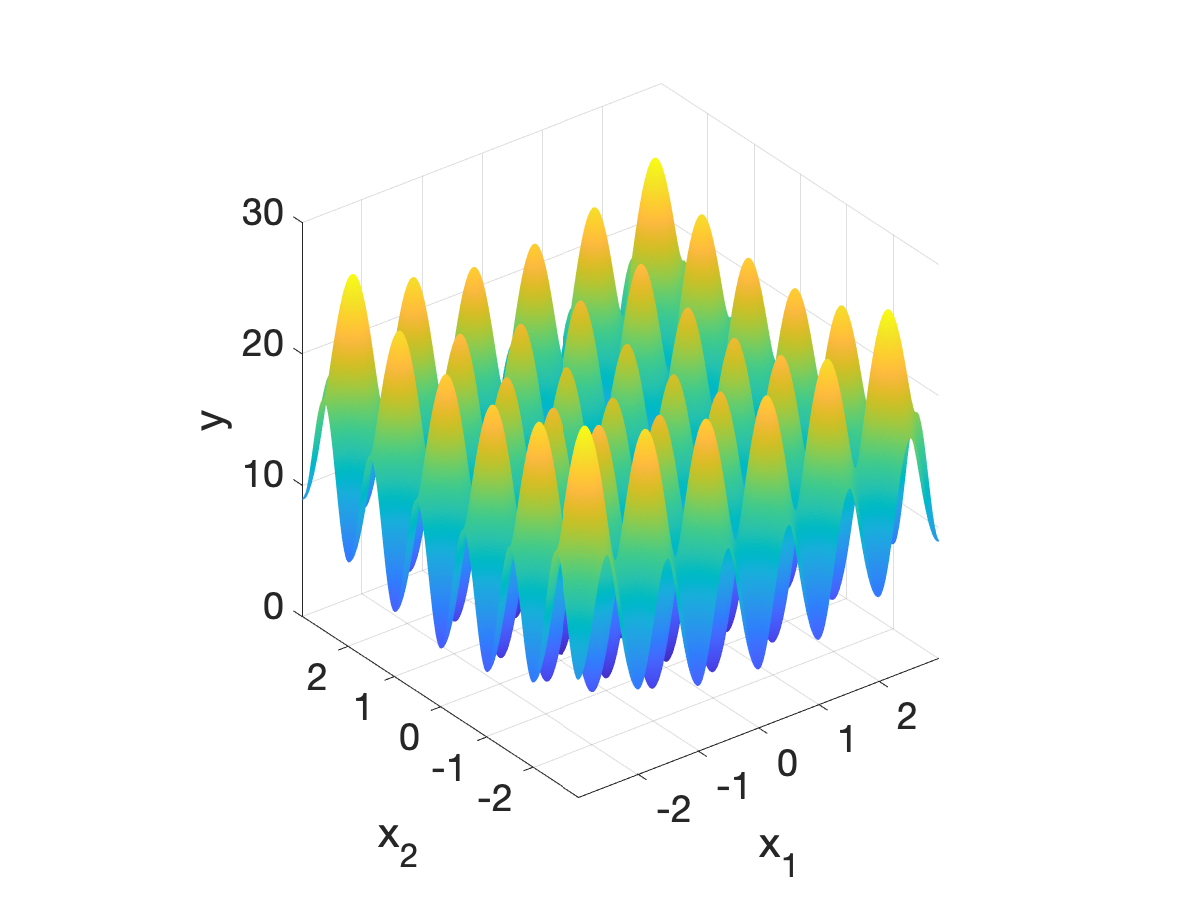
\includegraphics[width=1.1\linewidth]{Figure/R_function}
	%\caption{$d=2$ and $B=C=0$}
	\end{figure}
\end{columns}
\end{frame}

\begin{frame}
\frametitle{Massive local minima of Rastrigin function}

\begin{itemize}
	\item Exponential growth of the number of local minima: $5^d$
	\item Number of minima is $5^{1000}\approx 10^{690}$, when $d=1000$
	\begin{table}[ht]
		
		\centering\begin{tabular}{|c|c|c|c|c|c|}
			\hline
			d & 1 & 2 & 30 & 100 & 1000 \\
			\hline
			Number of local minima & $5$ & $5^2$ & $5^{30}$ & $5^{100}$ & $5^{1000}$\\
			\hline 
		\end{tabular}
		\caption{Number of local minima in terms of dimension}
	\end{table}
\end{itemize}

\end{frame}

\begin{frame}
\frametitle{Comparison with different random processes}
\begin{table}
	\centering
	\begin{tabular}{|c|c|c|c|c|c|}
		\hline
		\multirow{2}*{$d$}&
		\multirow{2}*{$N$}&
		\multirow{2}*{$M$}&\multicolumn{3}{c|}{CBO}\\
		\cline{4-6}
		~& ~ & ~ &  $\mathcal{N}(0,1)$&$\mathcal{U}(-1,1)$ &Wiener process  \\
		\hline 
		2  & 50 & 40 & 100\% & 100\% & 99\% \\
		10 & 50 & 40 & 100\% & 100\% & 2\%  \\
		20 & 50 & 40 & 98\%  & 22\%  & 0\%  \\
		20 & 50 & 20 & 66\%  & 2\%   & 0\%  \\
		30 & 50 & 40 & 26\%  & 0\%   & 0\%  \\
		30 & 500&5   &  0\%  & 0\%   & 0\%  \\
		%30 & 500 & 400 &     & 0\%   &  \%  \\
		\hline
		\multirow{2}*{$d$}&
		\multirow{2}*{$N$}&
		\multirow{2}*{$M$}&\multicolumn{3}{c|}{Adam-CBO}\\
		\cline{4-6}
		~& ~ & ~ &  $\mathcal{N}(0,1)$& $\mathcal{U}(-1,1)$ &Wiener process  \\
		\hline
		30 & 500  & 5  & 99\% & 100\% & 0\% \\
		100& 5000 & 5  & 100\% & 100\% & 0\%\\
		1000& 8000 & 50 & 92\% & 20\% &0\%\\
		\hline
	\end{tabular}
\end{table}	
\end{frame}
\begin{frame}
\frametitle{$\lambda = 0.1$, and $\sigma^t= 0.99^{\frac{t}{20}}$}

\begin{table}
	\centering
	\begin{tabular}{|c|c|c|c|c|}
		\hline
		\multirow{2}*{$d$}&
		\multirow{2}*{$N$}&
		\multirow{2}*{$M$}&\multicolumn{2}{c|}{Adam-CBO}\\
		\cline{4-5}
		~& ~ & ~ &  $\mathcal{N}(0,1)$& $\mathcal{U}(-1,1)$\\
		\hline
		1000& 8000 &  50  & 92\% & 20\% \\
		1000& 10000 & 50  & 100\% & 28\% \\
		1000& 12000 & 50  & 100\% & 28\% \\
		1000& 14000 & 50  & 100\% & 32\% \\
		1000& 16000 & 50  & 100\% & 32\%  \\
		\hline
	\end{tabular}
	%\caption{Different numbers of particles when the dimension is $1000$}
	\label{tbl:p_N sr}
\end{table}

\end{frame}
\subsection{Machine learning tasks}
\begin{frame}
\frametitle{Spectrail bias \cite{Rahaman2018}/Frequency principle \cite{xu2019frequency}}

	\begin{columns}
	\column{0.5\textwidth}
	
	\begin{itemize}
		\item[] \begin{align*}
		u(x) = \sin(2\pi x) + \sin(8 \pi x ^2)
		\end{align*}
		\item Network width $ = 50$, depth $ = 3$, and $2701$ parameters 
		\item $\lambda=0.2$
		\item $N = 500$ and $M=5$ in the first $50000$ iterations
		\item Afterwards the random term is ignored and $M = 10$
	\end{itemize}
	
	\column{0.5\textwidth}
	\begin{figure}[ht]
		\centering
		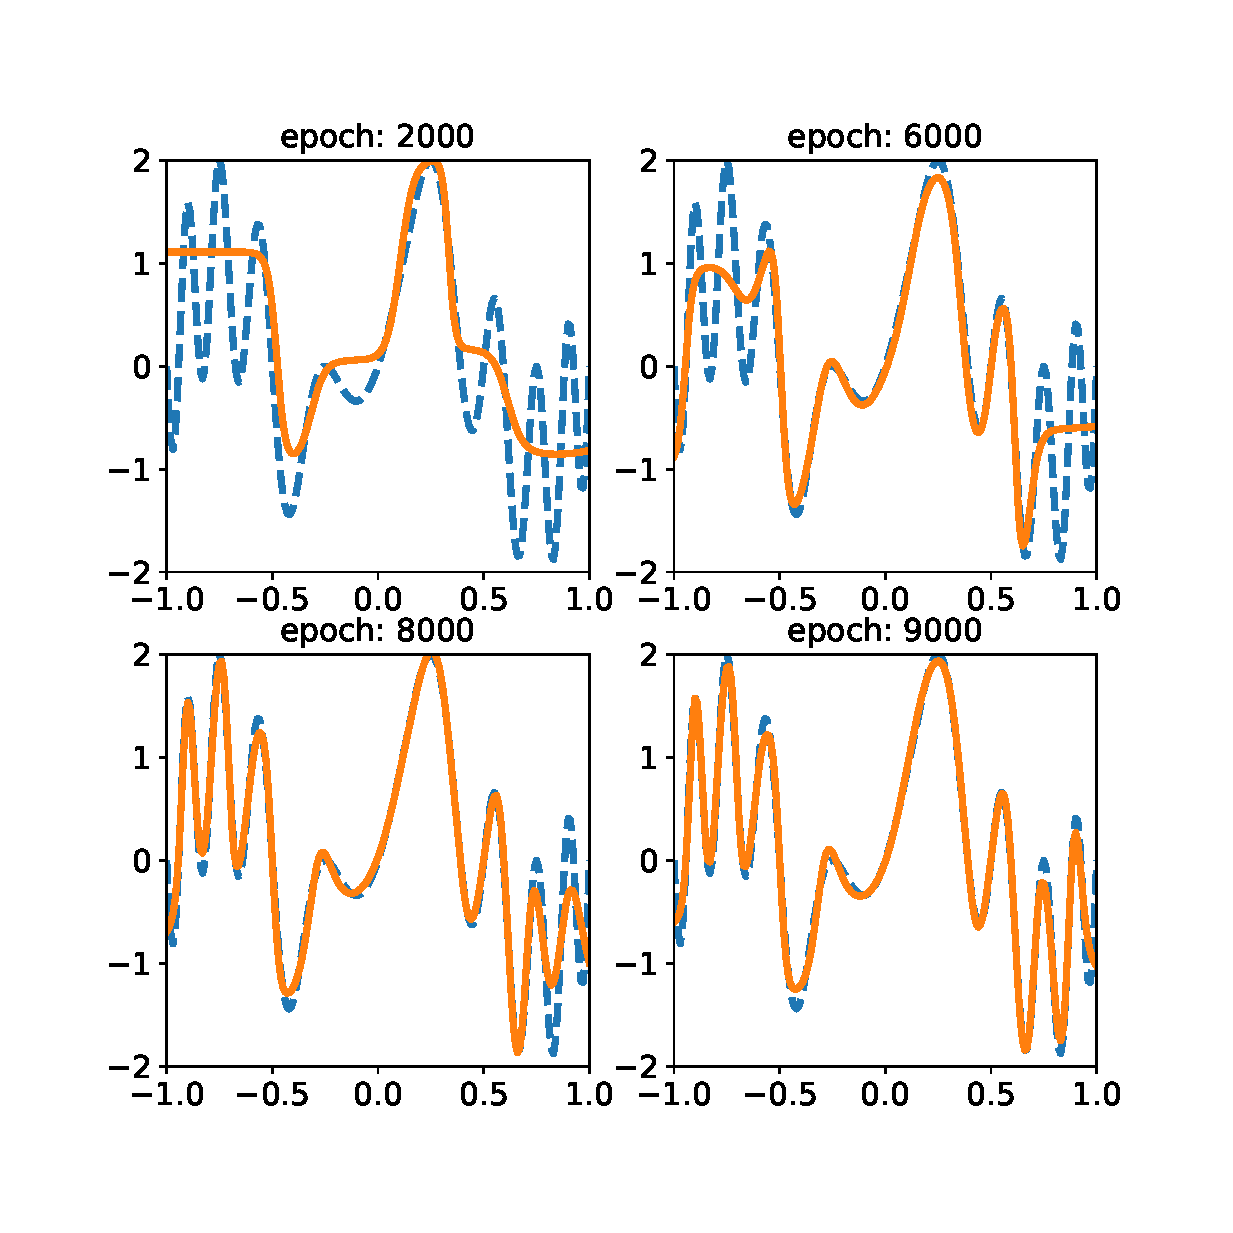
\includegraphics[width=0.7\linewidth]{Figure//Fprinciple_exm1}
	\end{figure}	
	\end{columns}

\end{frame}
\begin{frame}
\begin{columns}
\column{0.5\textwidth}
	\begin{align*}
	&u(x) = \left\{\begin{matrix}
	1   & x < -\frac{7}{8}, x> \frac{7}{8}, -\frac{1}{8}<x<\frac{1}{8}\\
	-1  & \frac{3}{8}< x< \frac{5}{8} , -\frac{5}{8}< x<- \frac{3}{8}\\
	0 & \text{otherwise} 
	\end{matrix} \right.
	\end{align*}
	The same setup as in the previous slide
	\column{0.5\textwidth}
	\begin{figure}[ht]
		\centering
		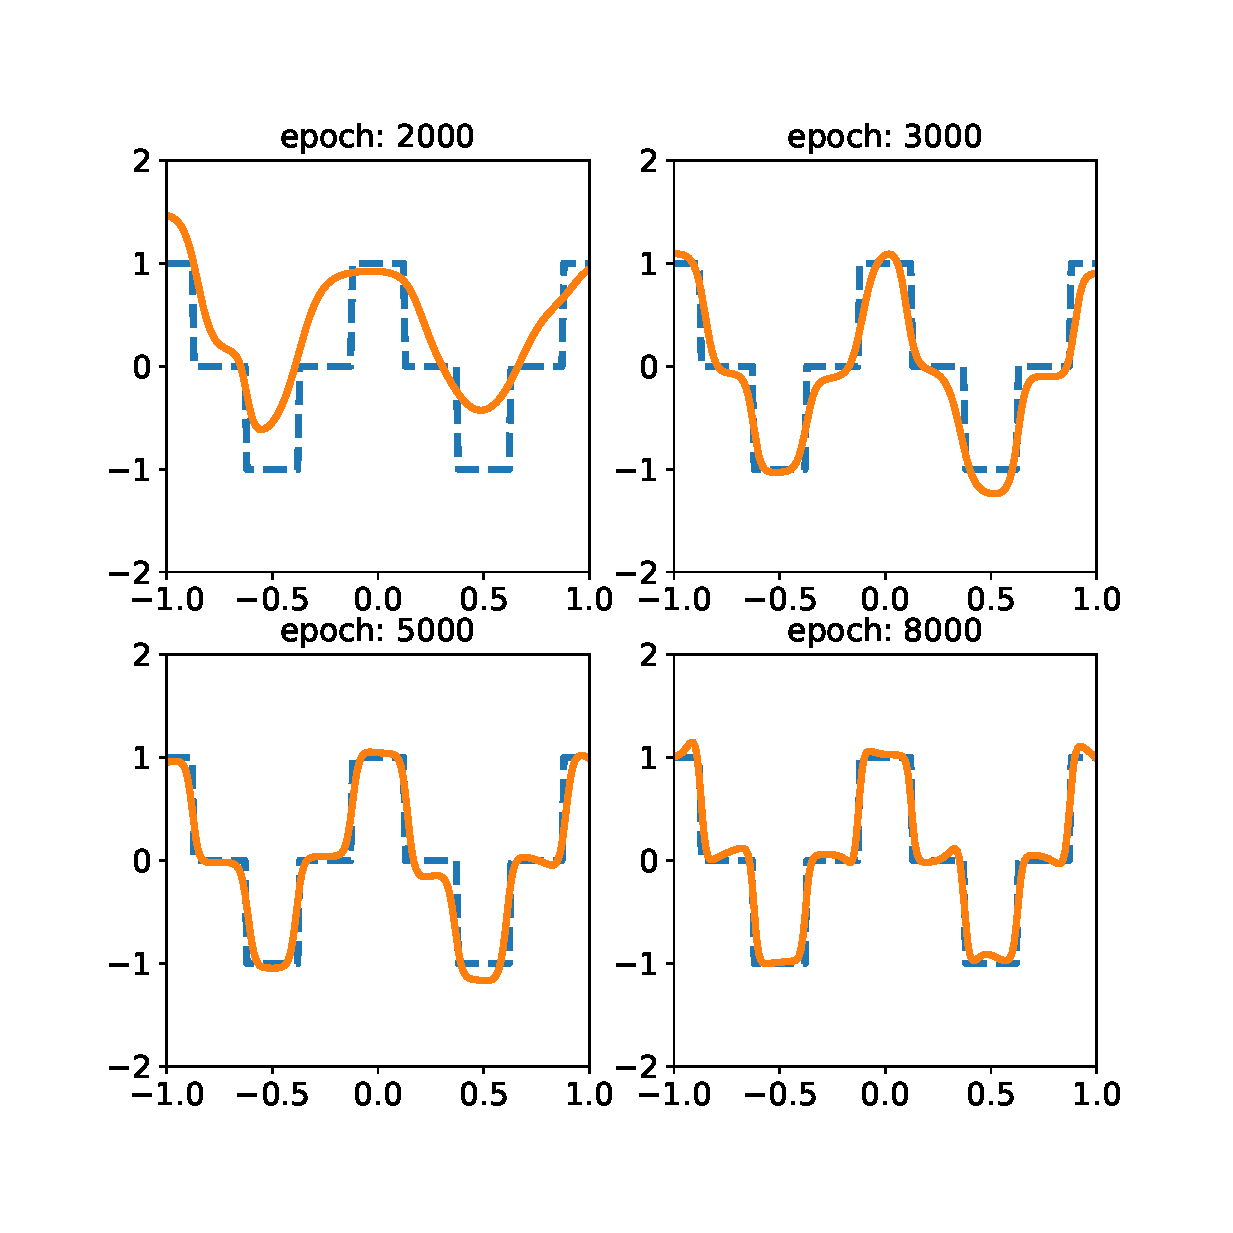
\includegraphics[width=0.7\linewidth]{Figure//Fprinciple_exm2}
	\end{figure}		
\end{columns}
\end{frame}
\begin{frame}
\frametitle{Gradient exploding or vanishing: DNN with fixed width $10$ and different depths}

\begin{equation*}
	u(x) = \sin(k\pi x ^k)
\end{equation*} 
$N = 500$, $M = 5$
\begin{table}
	\centering
	\begin{tabular}{|c|c|c|c|c|}
	\hline
		 depth & Num of parameters & k = 2 &  k = 3 & k = 4  \\
		\hline
		4   & 141 & 6.62 e-03 & 1.32 e-02 & 1.71 e-01\\
		7   & 471 & 4.78 e-03 & 1.42 e-02 & 7.54 e-03\\
		12  & 1021 & 7.44 e-03 & 1.30 e-02 & 5.32 e-02\\
		22  & 2121 & 1.00 e-02 & 1.01 e-02 & 1.21 e-01\\
		\hline
	\end{tabular}
	\caption{Absolute $L^2$ norm in terms of network depth when $k=2, 3, 4$}
\end{table}	

SGD or Adam fails to converges well (with final error around $0.3$) when the network depth is $4$ and $10$, respectively

\end{frame}

\begin{frame}
\frametitle{Solving PDEs by DNNs: Deep Ritz method \footfullcite{weinan2018deep}}

\begin{equation*}
\left\{
\begin{aligned}
&-\nabla \cdot ( A(x) \nabla u) = - \sum_{i=1}^d\delta(x_i) & x\in \Omega=[-1,1]^d\\
&u(x) = g(x)  & x\in \partial \Omega
\end{aligned}\right.
\end{equation*} 
with
\begin{equation*}
	A(x)= 
	\left[\begin{matrix}
		(x_1^2)^{\frac{1}{4}} & & \\
		& \ddots & &\\
		& &  (x_d^2)^{\frac{1}{4}}
	\end{matrix}\right].
\end{equation*}
\begin{itemize}
	\item Exact solution $u(x)= \sum_{i=1}^d|x_i|^{\frac{1}{2}}$ is only in $H^{1/2}(\Omega)$ 
	\item Derivatives have singularities at $x_i =0$
\end{itemize}

\end{frame}
\begin{frame}
\frametitle{Loss function in Deep Ritz method}

\begin{equation*}
\begin{aligned}
	I[u] =& \int_{\Omega}\frac{1}{2}(\nabla u)^T  A(x)  \nabla u(x)\mathrm{d}x + \sum_{i=1}^d\int_{-1}^{1}\delta(x_i)u(x)\mathrm{d}x_i \\ & + \eta \int_{\partial \Omega} (u(x)-g(x))^2 \mathrm{d}x,
	\end{aligned}
\end{equation*}	
\tiny{
\begin{table}[H]
	\centering
	\begin{tabular}{|c|c|c|c|c|c|}
		\hline
		d & n & m &  Activation-Optimizer & $L^2$ error & $L^{\infty}$ error\\
		\hline
		\multirow{4}*{2}&\multirow{4}*{20} & \multirow{4}*{2} & ReLu-Adam & 1.23 e-02 & 9.91 e-02\\
		& &  & ReQu-Adam & 2.22 e-02  & 4.21 e-01 \\
		& &  & sigmoid-Adam & 2.19 e-02 & 3.14 e-01\\
		& &  & $|x|^{0.5}$ - Adam-CBO & 3.96 e-03 & 2.09 e-02\\
		\hline
		\multirow{4}*{4}&\multirow{4}*{40} & \multirow{4}*{2} & ReLu-Adam & 6.72 e-03 & 3.70 e-01\\
		& &  & ReQu-Adam & 1.43 e-02 & 1.10 e -00\\
		& &  & sigmoid-Adam & 7.90 e-03 & 7.66 e -02\\
		& &  & $|x|^{0.5}$ -Adam-CBO & 3.13 e-03 & 9.52 e -02\\
		\hline
	\end{tabular}
\caption{Errors in $L^2$ and $L^{\infty}$ norms by Adam and Adam-CBO methods}
\end{table}	
}
\end{frame}

\begin{frame}
\frametitle{Cont'd}

	\begin{figure}
	\subfigure[$L^{\infty}$ error]{
		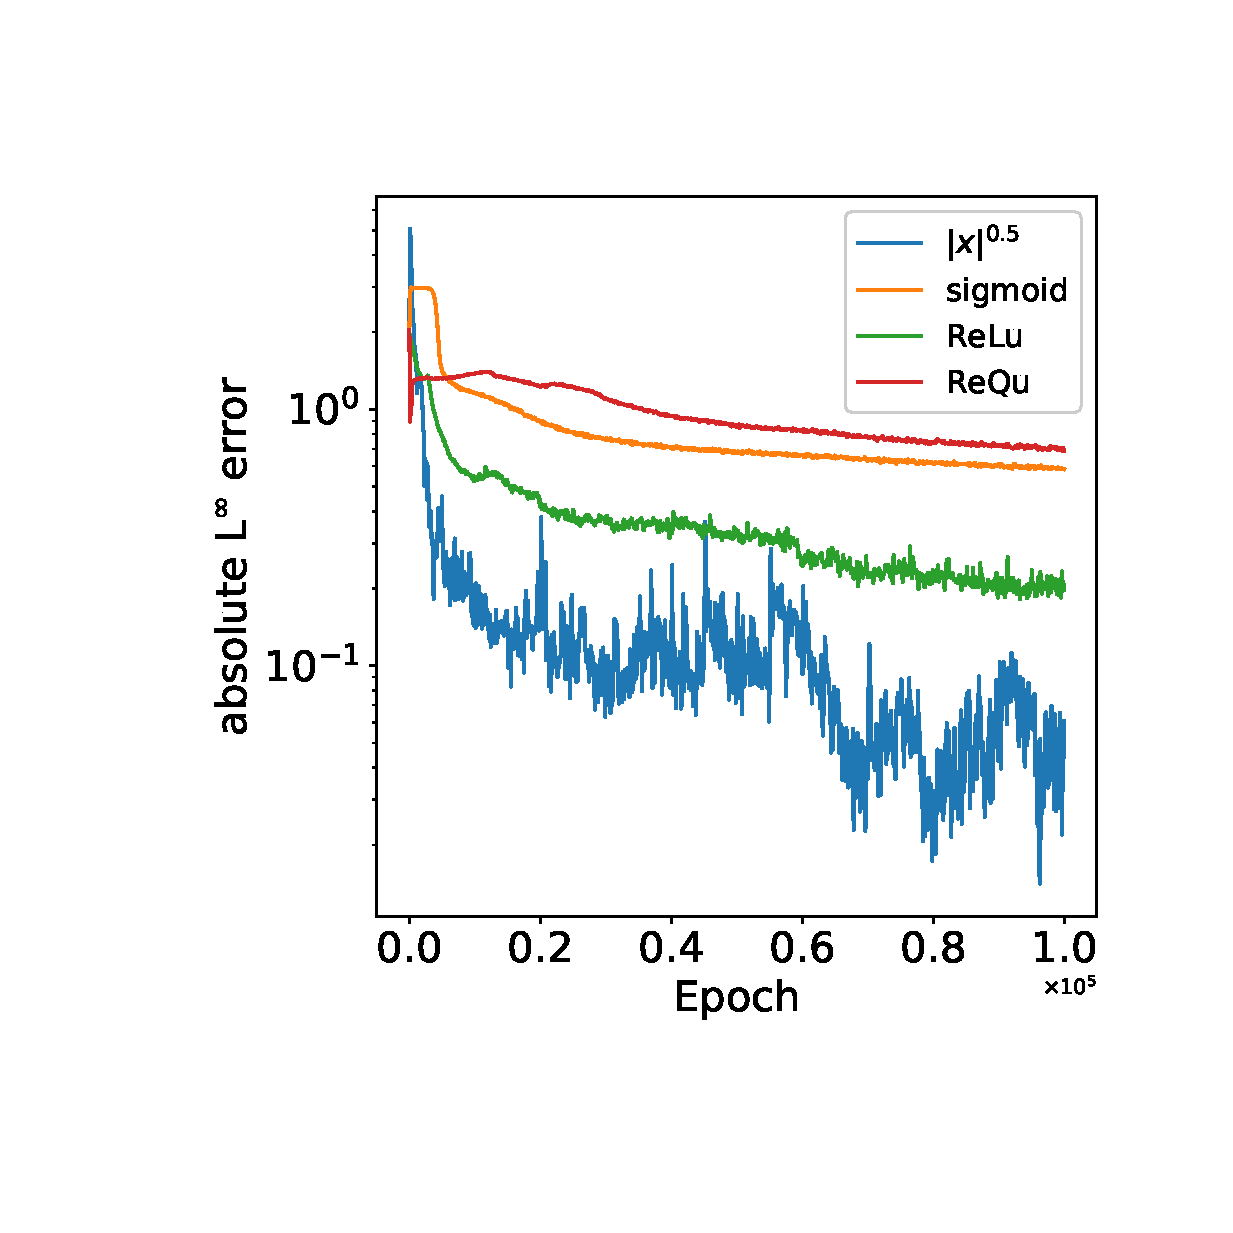
\includegraphics[width=0.45\linewidth]{Figure//singular_PDE_4D_L_infty_error}
	}
	\subfigure[$L^2$ error]{
		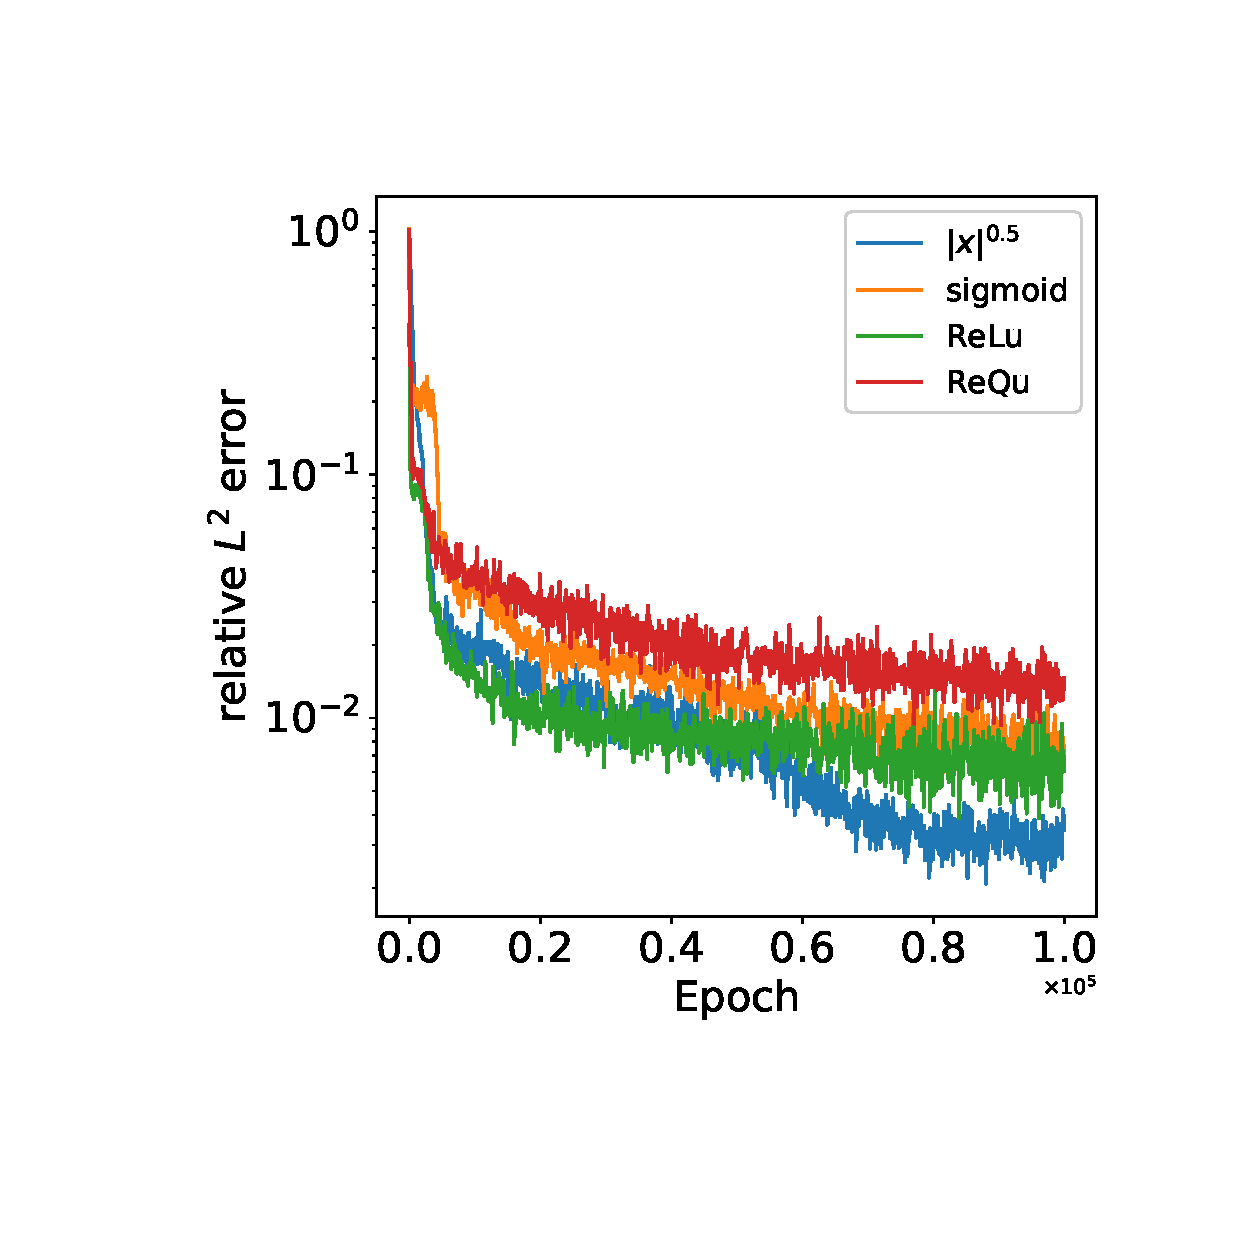
\includegraphics[width=0.45\linewidth]{Figure//singular_PDE_4D_L2_error}
	}
	\caption{Training process of Adam and Adam-CBO methods when $d=4$}
\end{figure}

\end{frame}
\begin{frame}
\frametitle{Singularities}

\begin{figure}
	\subfigure[$x_2=x_3=x_4=0$]{
		\includegraphics[width=0.45\linewidth]{Figure//singular_PDE_4D_Landscape_x1}
	}
	\subfigure[$x_1=x_3=x_4=0$]{
		\includegraphics[width=0.45\linewidth]{Figure//singular_PDE_4D_Landscape_x2}
	}
	\caption{One-dimensional solution profiles at the intersection}
\end{figure}	
\end{frame}

\begin{frame}
\frametitle{Conclusion}

Adam-CBO is
\begin{itemize}
	\item able to find the global minimizer in high dimensions
	\item free of curse of dimensionality
	\item suitable for machine learning tasks with
	\begin{itemize}
		\item gradient explosion or vanishing
		\item non-different activation functions
	\end{itemize}
\end{itemize}
{\huge\medskip
\begin{center}
	Thank you for your attention!
\end{center}
}
\end{frame}

\end{document}
